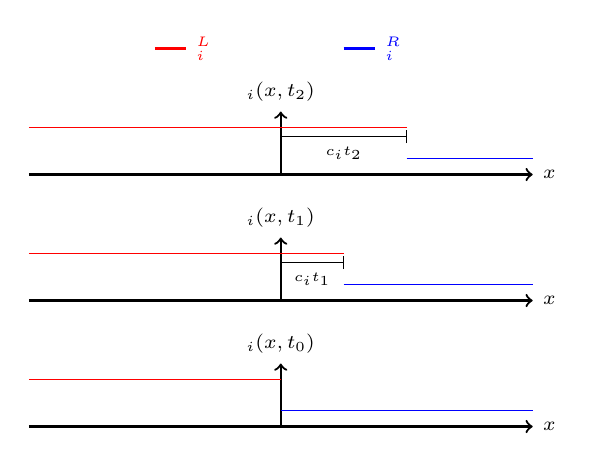
\begin{tikzpicture}[scale=0.8]
  %% t2
  \draw[->,thick] (0,0) -- (0,1) node [above] {\scriptsize$\Pc_i(x,t_2)$};
  \draw[->,thick] (-4,0) -- (4,0) node [right] {\scriptsize$x$};
  \draw[Blue] (2,0.25) -- (4,0.25);
  \draw[Red] (-4,0.75) -- (2,0.75);
  \draw (0,0.6)--(2,0.6) node [midway, below] {\tiny $c_it_2$};
  \draw (2,0.5)--(2,0.7);
  %% t1
  \draw[->,thick] (0,-2) -- (0,-1) node [above] {\scriptsize$\Pc_i(x,t_1)$};
  \draw[->,thick] (-4,-2) -- (4,-2) node [right] {\scriptsize$x$};
  \draw[Blue] (1,0.25-2) -- (4,0.25-2);
  \draw[Red] (-4,0.75-2) -- (1,0.75-2);
  \draw (0,0.6-2)--(1,0.6-2) node [midway, below] {\tiny $c_it_1$};
  \draw (1,0.5-2)--(1,0.7-2);
  %% t0
  \draw[->,thick] (0,-4) -- (0,-3) node [above] {\scriptsize$\Pc_i(x,t_0)$};
  \draw[->,thick] (-4,-4) -- (4,-4) node [right] {\scriptsize$x$};
  \draw[Blue] (0,0.25-4.) -- (4,0.25-4.);
  \draw[Red] (-4,0.75-4.) -- (0,0.75-4.);
  %% legend
  \draw[thick,Red] (-2.,2.) -- (-1.5,2.) node [right] {\scriptsize$\Pc_i^L$};
  \draw[thick,Blue] (1,2.) -- (1.5,2.) node [right] {\scriptsize$\Pc_i^R$};
\end{tikzpicture}
%%% Local Variables:
%%% mode: latex
%%% TeX-master: "../../mainManuscript"
%%% End: